%!tex program = lualatex
\documentclass{ctexart}
\usepackage{graphicx}
\usepackage[margin=2cm]{geometry}
\usepackage{amsmath}
\usepackage{amssymb}
\usepackage{tikz}
\usetikzlibrary{calc, patterns, intersections}
\pagestyle{empty}
\newcounter{xcord}
\newcounter{ycord}
\newcounter{total}
\ctexset{
	subsection/name = {第,题},
	subsection/number = {\thesubsection},
	section ={
		name = {第,部分}
	}
}
\renewcommand{\labelenumi}{\textbf{\ifnum\value{enumi}<10 0\fi\arabic{enumi})}}
\begin{document}
\section{求阴影面积}
\begin{figure}[htbp]
	\centering
	\begin{gather*}
		长方形ABCD\\
		AB = 9 \\
		BC = 6 \\
		求阴影面积
	\end{gather*}
	\begin{tikzpicture}[scale=.5]
		\coordinate (A) at (9,0);
		\coordinate (B) at (0,0);
		\coordinate (C) at (0,-6);
		\coordinate (D) at (9, -6);
		\coordinate (E) at (3, 0);
		\coordinate (F) at (5, -6);
		\coordinate (C') at (9, -3);
		\coordinate (B') at ($(C') ! 1.2 ! -90:(F)$);
		\path [name path=B'C'] (B') -- (C');
		\path [name path=AE] (A) -- (E);

		\draw [name intersections={of=B'C' and AE, by=G}];
		\node [above right] at(G){$G$};

		% \path[draw=red] {AE};

		\draw[dashed](B) -- (E);
		\draw (E)-- (A) -- (D) -- (F) -- (E);
		\draw[dashed] (F) -- (C) -- (B);
		\draw (F) -- (C') -- (B') -- (E);

		\draw [pattern=north east lines](E) -- (G) -- (C') -- (F) -- cycle;
		\node at (A)[above right]{$A$};
		\node at (B)[above left]{$B$};
		\node at (C)[below left]{$C$};
		\node at (D)[below right]{$D$};
		\node at (F)[below]{$F$};
		\node at (C')[right]{$C\prime$ 中点};
		\node at (E)[above left]{$E$};
		\node at (B')[right, xshift=5pt]{$B\prime$};
	\end{tikzpicture}
\end{figure}

\begin{align}
	FC + FD                    & = 9                      \\
	FC^2                       & = FD^2 + DC^2 = FD^2 + 9 \\
	(FC + FD) \times (FC - FD) & = 9                      \\
	FC - FD                    & = 1                      \\
	FC                         & = 5
\end{align}

Calculate the length of $BE$:
\begin{align}
	\triangle CDF            & \approx \triangle CAG                               \\
	\frac{GA}{AC}            & = \frac{CD}{FD} = \frac{3}{4}                       \\
	GA                       & = \frac{9}{4}                                       \\
	GC                       & = \sqrt{GA^2 + AC^2} = \frac{15}{4}                 \\
	BG                       & = BC - GC = 6 - \frac{15}{4}     = \frac{9}{4} = GA \\
	\because \triangle GBE   & \approx \triangle GAC                               \\
	\therefore \triangle GBE & \cong \triangle GAC                                 \\
	BE                       & = AC = 3
\end{align}

\section*{20以内两位数乘法练习}
\begin{center}
	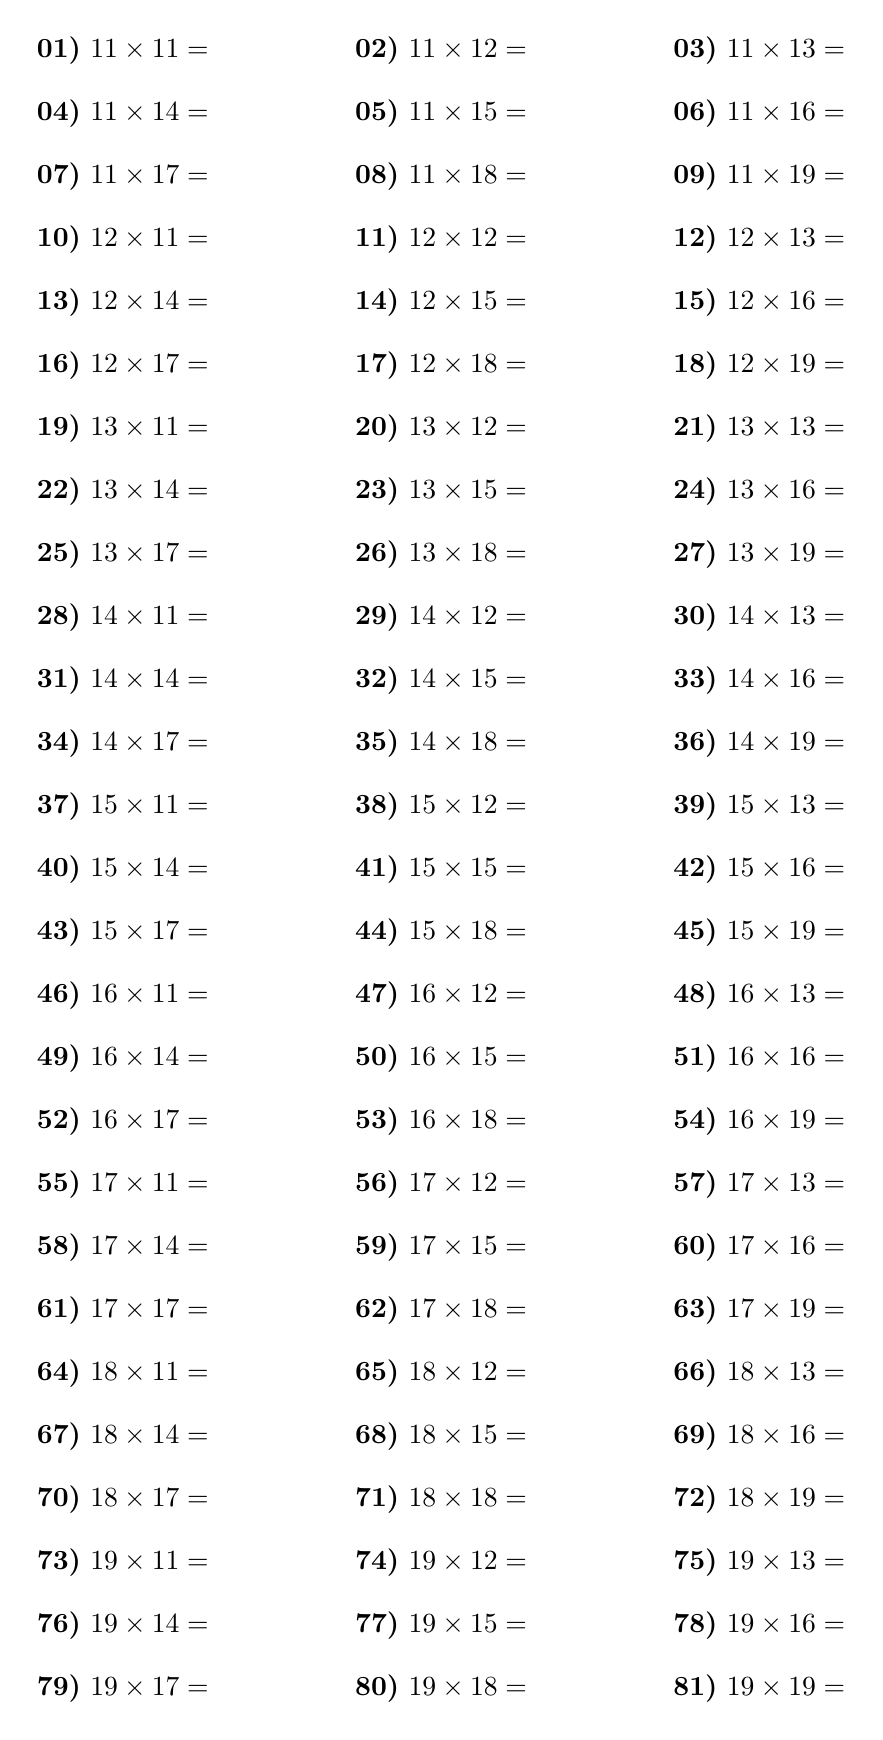
\begin{tikzpicture}
		\foreach \x in {11,...,19}
		\foreach \y in {11,...,19}
			{
				\stepcounter{total}
				\node at (\value{xcord} * \textwidth / 3, -\value{ycord}*0.8) {\textbf{\ifnum\value{total}<10
				0\fi\thetotal)} $\x \times \y =$};
		\stepcounter{xcord}		\ifnum\value{xcord}=3
		\setcounter{xcord}{0}
		\stepcounter{ycord}
		\fi
		}
	\end{tikzpicture}

\end{center}

\section{速算及巧算}
\subsection{计算总和}
\begin{enumerate}
	\item $1-2+3-4+5-6+7-8+9-10+11=$

	\item $3+5+7+9+11+13+15+17+19+21=$

	\item $100-99+98-97+96-95+94-93+93-92+91=$

	\item $6+8+10+12+14+16+18+20+22+24=$

	\item $1 + 2 + 3 + \ldots + 100 = $

	\item $2 + 4 +6 + \ldots + 100 = $

	\item $1 + 3 + 5 + \ldots + 99 = $

	\item $5 + 10 + 15 + \ldots + 100 = $

	\item $1 - (1+2) + (1+2+3) - (1+2+3+4) + \ldots - (1+2+\ldots+98) + (1+2+\ldots+99) = $

	\item $1-2+3-4+\ldots+2023-2024+2025=$

	\item $19+28+37+46+55+64+73+82+91+ \underline{\hspace{1cm}}=550$

	\item $2000-180+220-180+220-180+220-180+220-180+220=$

	\item $352.46-35.58-65.93-76.07-24.42=$

	\item $1+2+4+8+16+32+64+128+256+512+1024=$

	\item $8+89+899+8999+89999=$

	\item $8+88+888+8888+88888=$

	\item $28+208+2008+20008=$

	\item $24+63+52+17+49+81+74+38+95=$

	\item $1999.9+199.9+19.9+1.9=$

	\item $(7+9+11+13+\ldots+37)-(9+11+13+15+\ldots+35)=$

\end{enumerate}

\pagebreak
\section{速算和巧算2}

\begin{enumerate}

	\item $(6+8+10+12+\ldots+36)-(8+10+12+14+\ldots+34)=$

	\item $(1+4+7+10+\ldots+40)-(4+7+10+13+\ldots+37)=$
\end{enumerate}

\section{SVSU2022 level1}
\begin{questions}
	\question 考虑方程$p(x): ax^2 + bx + c=0$,其系数$a$,$b$和$c$都是非零的,并且每个系数都满足从方程$p(x)$
	中移除包含该系数的项后得到的方程;例如,系数$b$是方程 $ax^2+c=0$的一个解。求方程$p(x)$
	所有解的和是多少?

	\begin{oneparchoices}
		\CorrectChoice 总是 1 \choice 总是 -1 \choice 总是 2 \choice 1 或者 -1 \choice 1 或者 2
	\end{oneparchoices}
	\begin{solution}
		方程$p(x)$的两个解分别为$\displaystyle x_1, x_2 = \frac{-b \pm \sqrt{b^2 - 4ac}}{2a}$,则$\displaystyle x_1 +
			x_2 = -\frac{b}{a}$\\
		由题意得
		\begin{align}
			ac^2  + bc & = 0 \label{\thequestion:1} \\
			ab^2  + c  & = 0 \label{\thequestion:2} \\
			ab    + c  & = 0 \label{\thequestion:3}
		\end{align}
		由式(\ref{\thequestion:2}) 和(\ref{\thequestion:3})得$b=1$和$a+c=0$,代入(\ref{\thequestion:1})得:
		\begin{equation}
			a(-a) -a  = 0
		\end{equation}

		则$a=-1$或$a=0$,因为题目中$a \ne 0$,所以$a=-1$,则$\displaystyle x_1 + x_2 = -\frac{b}{a}=1$
	\end{solution}
\end{questions}
\section{SVSU2022 level2}
\subsection{}
求
$\displaystyle\sum_{k=0}^{2022}\frac{2022!\cdot (-1)^k2^k}{k! \cdot (2022-k)!}$
的值

\subsection*{解:}
\begin{enumerate}
	\item 利用二项式定理$\displaystyle(x+y)^n = \sum_{k=0}^{n}\binom{n}{k}x^ky^{n-k}$
	      \begin{align}
		      \sum_{k=0}^{2022}\frac{2022!\cdot(-1)^k2^k}{k!\cdot(2022-k)!} & = \sum_{k=0}^{2022}\frac{2022!}{k!\cdot
		      (2022-k)!}(-2)^k                                                                                        \\
		                                                                    & =
		      \sum_{k=0}^{2022}\binom{2022}{k}(-2)^k\cdot 1^{2022-k}                                                  \\
		                                                                    & = (1-2)^{2022}                          \\
		                                                                    & = 1
	      \end{align}
\end{enumerate}

\subsection{}
求$(\sqrt[4]{27} + \sqrt{3} + \sqrt[4]{3} + 1)^2$
\subsection*{解:}
\begin{enumerate}
	\item 设$\displaystyle x=3^{\frac{1}{4}}$,则
	      \begin{align}
		      (\sqrt[4]{27} + \sqrt{3} + \sqrt[4]{3} + 1)^2 & = (x^3 + x^2 + x + 1)^2                     \\
		                                                    & = [x^2(x+1) + (x+1)]^2                      \\
		                                                    & = (x^2 + 1)^2(x+1)^2                        \\
		                                                    & = \frac{(x^2 + 1)^2(x+1)^2(x-1)^2}{(x-1)^2} \\
		                                                    & = \frac{(x^4 - 1)^2}{(x-1)^2}
	      \end{align}
	\item 将$x=\sqrt[4]{3}$代入得:
	      \begin{align}
		      \frac{(x^4 - 1)^2}{(x-1)^2} & = \frac{4}{(x-1)^2}                     \\
		                                  & = \frac{4}{x^2 - 2x + 1}                \\
		                                  & = \frac{4}{\sqrt{3} - 2\sqrt[4]{3} + 1}
	      \end{align}
\end{enumerate}

\end{document}
